\subsection{Ερώτημα iv}
   \begin{minipage}{\textwidth}
      \begin{center}
         \fbox{\textlatin{\textbf{\textit{Kaby Lake Microarchitecture}}}}\\
         \vspace{3mm}
         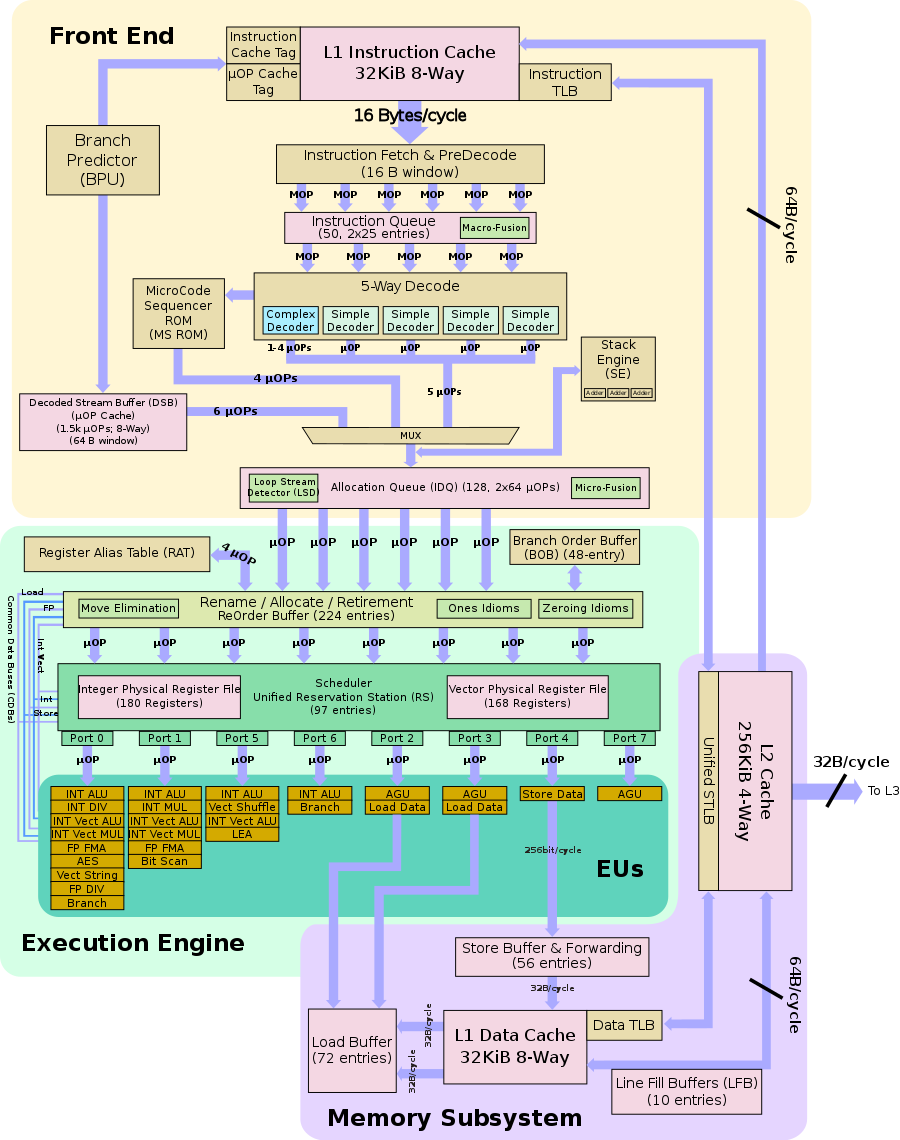
\includegraphics[width=\textwidth]{./imgs/kaby.png}
         \vspace{6mm}
      \end{center}
   \end{minipage}

   Για τον προσωπικό μου υπολογιστή / latpop, ο επεξεργαστής του Intel Core 
   \textbf{i7-8550U}
   χρησιμοποιεί την αρχιτεκτονική Kaby Lake.
   (https://en.wikichip.org/wiki/intel/microarchitectures/kaby\_lake).

   Όπως φαίνεται στο διάγραμμα, η αρχιτεκτονική Kaby Lake χρησιμοποιεί ReOrder
   Buffer με 224 entries (window size) και Dispatch Width = 6 εντολές. Σύμφωνα
   με την ανάλυση που προηγήθηκε, η επιλογή των χαρακτηριστικών αυτών είναι
   απολύτως λογική και δικαιολογητέα, αφού επιτυγχάνει αρκετά καλή απόδοση
   λαμβάνοντας υπ' όψιν το περιορισμένο μέγεθος chip και την χαμηλή κατανάλωση
   ενέργειας, αφού πρόκειται για επεξεργαστής προορισμένος για χρήση σε laptop. 
